\documentclass[10pt]{article}
\usepackage{graphicx,amsmath,amssymb,bm}
\usepackage{amsfonts}

\begin{document}

\section*{Mastergrads prosjekt for Marte Julie S\ae tra i Computational Physics: Mekanismer bak Calcium-spikes i LGN internevroner i hjernen.}

Vegledere: Gaute Einevoll (M) UMB og FI@UiO, Marianne Fyhn (M) IBV@UiO,  og Morten Hjorth-Jensen (H), FI@UiO. \newline

\subsection*{Introduksjon} 
Internevronet i LGN (LGN st\aa r for Lateral geniculate nucleus, en del av syns-thalamus i hjernen) genererer
en type respons som kalles {\em bursts}. Et {\em burst} er en serie med
tettkommende aksjonspotensialer (se Fig.~1A nedenfor). I Fig.~1A ble et
burst framprovosert gjennom \aa\ injisere en kort (10 ms), sterk
str\o mpuls inn i soma til et internevron. Som figuren viser, varte
responsen ('burstet') mye lenger (~100 ms) enn injeksjonen, noe som
tyder p\aa\ at en relativt treg aktiv mekanisme var involvert. Man kan se
denne mekanismen i isolasjon i kurven under (fortsatt Fig. 1A). Der
vises det samme eksperimentet, men i dette tilfellet ble
virkningsspotensialene (action potentials, heretter AP) blokkerte med et stoff som heter
TTX. Humpen man kan se etter stimulus-stans, kalles en 'Ca-spike',
fordi den er generert av Ca-kanaler. Ca-spike amplituden overskrider
ofte fyringsterskelen for APer, slik at disse burstene av APer,
vanligvis ligger p\aa\ toppen av Ca-spikes.

Internevronet i LGN har (minst) to typer ulike Ca-kanaler, som
kalles $T$-type og $L$-type Ca-kanaler \cite{Munsch1997}. I nesten alle
artikler der det er skrevet om 'bursts' i internevronene, hevdes det
at det er $T$-kanalene som ligger bak, se for eksempel referansen 
\cite{Pape1994,Pape1995,Zhu1999,Broicher2007}. Modelleringen gjort av Halnes {\em et al}
\cite{Halnes2011} gir tilsvarende resultat.  De f\aa\ unntakene som er dokumentert finnes i artikkelen til
Acuna-Goycholea {\em et al} \cite{AcunaGoycholea2008}. Figur~1A er henta derfra. Der
viste man at burstet kunne elimineres gjennom \aa\ tilf\o re et stoff som
heter Nimodipine (gr\aa\ linje i Fig.~1A viser en tiln\ae rma passiv
respons på input). Nimodipin er et stoff som brukes for \aa\ blokkere
$L$-kanaler. Siden nimodipin eliminerte Ca-spiken, kan en tolke
eksperimentet at spiken er mediert av $L$-kanaler.

Det finnes i den eksperimentelle
litteraturen indikasjoner p\aa\ at b\aa de $T$- og $L$-kanaler er involvert i \aa\
lage Ca-spikes i internevroner. Vi kan tenke oss at de to kanaltypene
kan ha en viss funksjonell overlapp. 
Dette mastergradsprosjektet starter med f\o rst \aa\ kartlegge rollene 
til de to respektive kanaltypene
i generering av Ca-spikes.

Prosjektet starter med  en forenkla modell, som kun
inneholder de to aktuelle kanaltypene ($T$-kanaler og $L$-kanaler), i
tillegg til den tradisjonelle passive str\o mmen
(lekkasjestr\o mmen). Den f\o rste delen g\aa r da ut p\aa\ \aa\ dokumentere hvordan de
to ulike ionekanalene p\aa virker/kan p\aa virke modellresponsen til en kort
str\o minjeksjon. En veit ikke 
p\aa\ forh\aa nd hvor mye det er av de respektive ionekanalene. Dette er
parametere som skal varieres.
I modellen kan vi variere:
\begin{itemize}
\item Tettheten (mengden) av de respektive kanaltypene.
\item Hvilepotensialet til nevronet (manipuleres gjennom lekkasjestr\o mmen)
\item Evt. str\o minjeksjonen (amplitude og varighet).
\end{itemize}
Noen spørsm\aa l som en kan besvare er
\begin{itemize}
\item	Hvilke aspekter av Ca-spikes p\aa virkes av de respektive kanaltypene? F.eks. kan det v\ae re slik at $T$-kanalene p\aa virker amplituden, mens $L$-kanalene drar ut varigheten til en Ca-spike?
\item Hvordan avhenger funnene over av nevronets hvilepotensial?
  Aktiveringa av kanalene er sterkt spenningsavhengig, og nevronets
  hvilepotensial vil v\ae re en avgj\o rende faktor. Dette kan variere
  fra $-70$ mV til $-60$ mV mellom ulike internevroner. Er det
  f.eks. slik at $T$-kanaler er viktige for responsen om nevronet hviler
  p\aa\ $-70$ mV, mens $L$-kanaler tar over i nevroner som hviler
  p\aa\ $-60$ mV?
\end{itemize}

Det endelige m\aa let er \aa\ bruke ekseperimentelle data sammen med
stokastiske optimerings verkt\o y for \aa\ kunne definere en mer
realistik modell ved \aa\ bygge p\aa\ Halnes {\em et al} sitt arbeid \cite{Halnes2011}. 
\begin{figure}[htb]
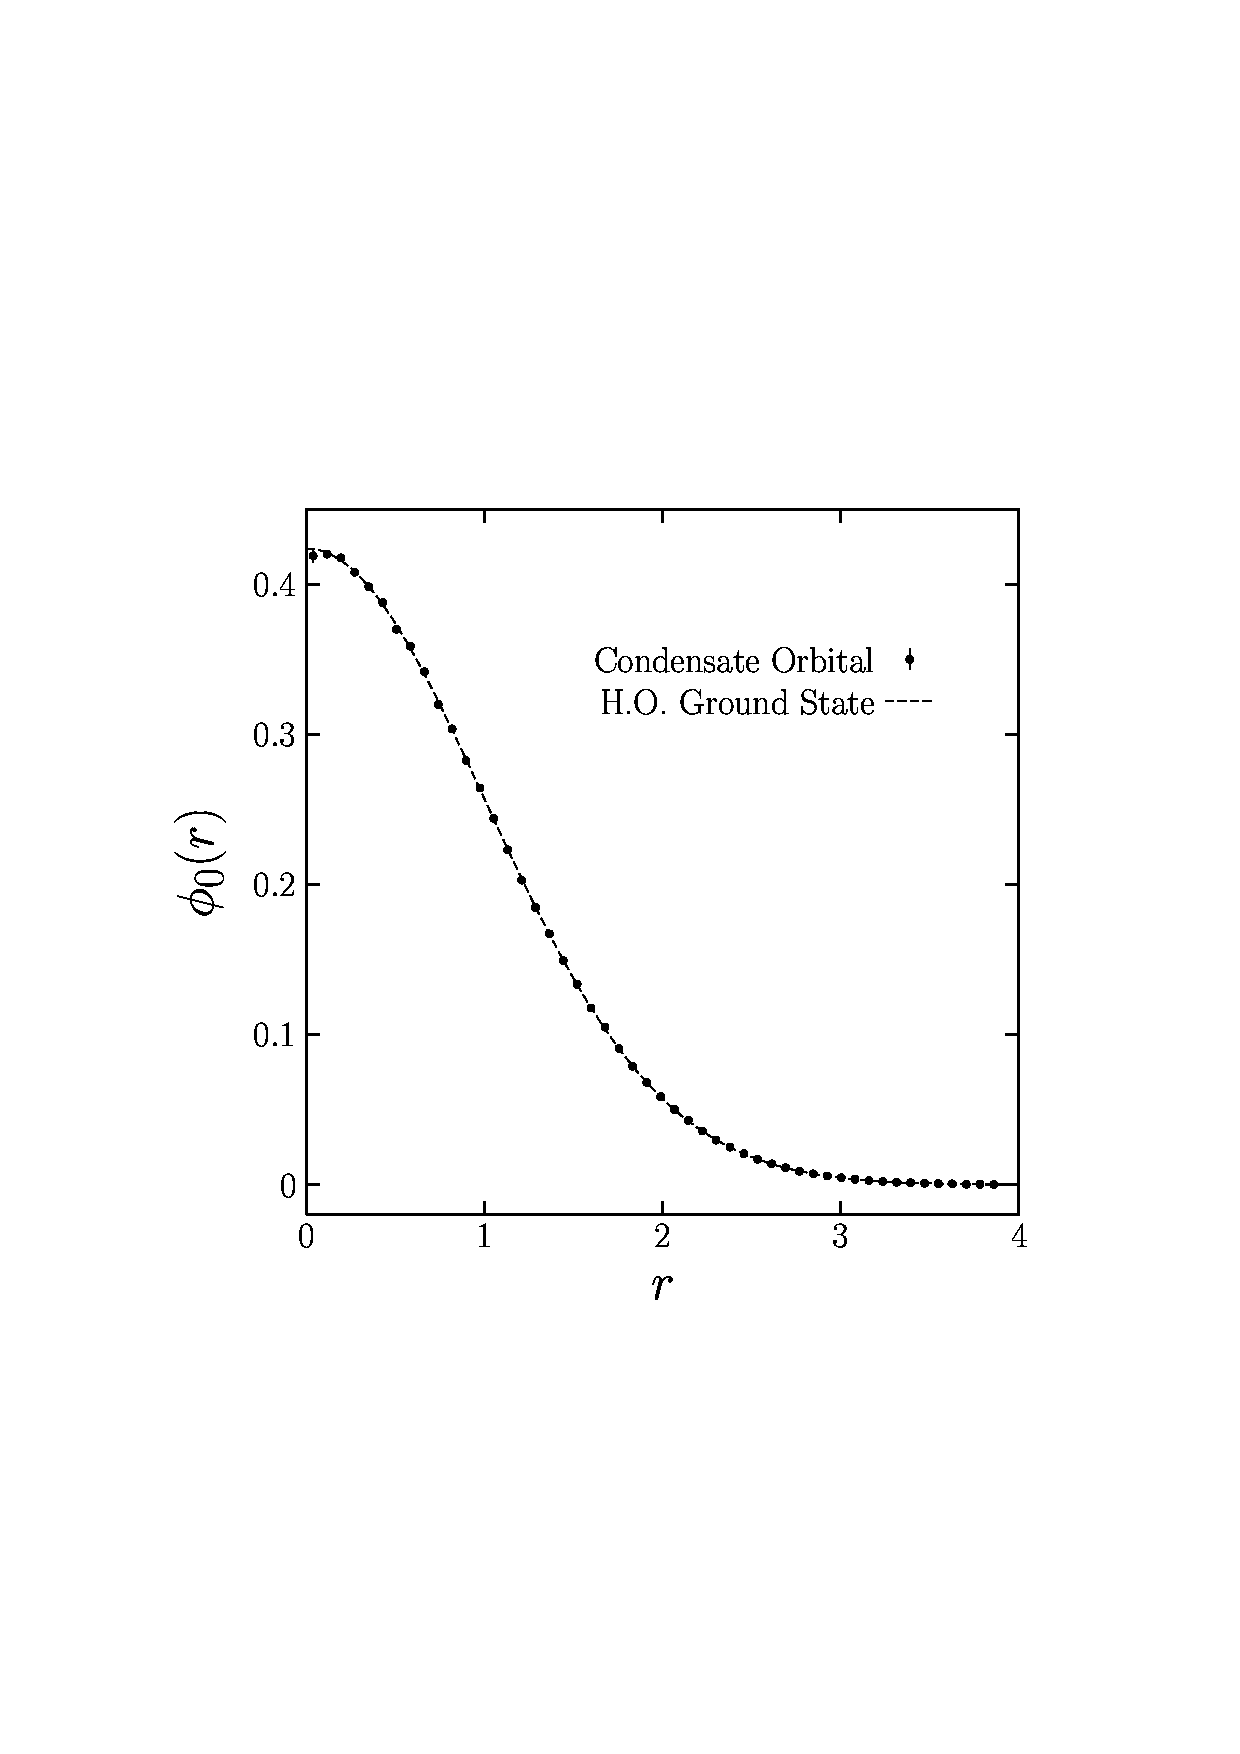
\includegraphics[width=1.0\textwidth]{fig1.png}
\caption{Calcium spikes i dLGN INs. Fra referanse~\cite{AcunaGoycholea2008}.}
\end{figure}

\subsection*{Modellering og prosjekt}

Simuleringene i  Fig.~1B viser noen preliminære simuleringer
fra Halnes {\em et al} sitt arbeid \cite{Halnes2011}. Modellen gis en strøminjeksjon
på 240 pA, og f\aa r en respons som likner eksperimentet i
Fig.~1A. Str\o minjeksjonen som m\aa tte til var noe h\o yere enn i
eksperimentet (180 pA), men siden membranresistansen varierer mellom
nevroner, er ikke dette noe \aa\ henge seg opp i. Figur 1C viser den
samme simuleringen i en forenklet modell. Der er alle 
ionekanaltyper bortsett fra $T$-kanalene og $L$-kanalene fjerna. I denne forenkla
modellen har Ca-spiken lengre varighet enn i originalen. Dette er
fordi originalen inneholder mekanismer som avbryter Ca-spiken noe
tidligere, og tvinger nevronet tilbake mot
hvilepotensialet. Kvalitativt sett, gir den forenkla modellen
likevel ganske greie resultater. I denne oppgava vil den brukes som  utgangspunkt
for \aa\ studere Ca-spikes.

For \aa\ kunne reprodusere \cite{Halnes2011} og anvende stokastiske optimeringsverkt\o y, er f\o rste steg \aa\ anvende de stokastiske optimeringsverkt\o ya p\aa\ den enkle modellen beskrevet ovafor. 
For \aa\ n\aa\ dette, vil modellkonstruksjonen inneholde f\o lgende steg:
\begin{enumerate}
\item	Et utgangspunkt kan v\ae re en standard implementering av Hodgkin-Huxley (HH) modellen. 
\item	Vi bytter ut Na og K-kanalene i HH-modellen, med tilsvarende beskrivelser for $T$- og $L$-kanaler. Disse kanalene er beskrevet med den samme formalismen som HH-kanalene. $T$- og $L$-kanalene vil bli de eneste komponentene i modellen som er direkte basert på internevronet, og kan tas fra internevronmodellen \cite{Halnes2011}.
\item En kan  
justere passivt reverseringspotensial for \aa\ f\aa\ riktig hvilepotensial i cella (f.eks. -63 mV) eller justere membranresistans for \aa\ f\aa\ noenlunde rimelige responser på str\o minjeksjon. For eksempel b\o r et kontinuerlig stimulus p\aa\ rundt 60 pA f\o re til at nevronet legger seg p\aa\ omtrent 40mV i steady state.
N\aa r det gjelder tetthetene av $T$- og $L$-kanaler kan vi begynne med verdiene fra \cite{Halnes2011}.
\item	Vi simulerer eksperimentet i Fig. 1A (dvs. bruker samme input til soma).
\item	Vi varierer tetthetene av $L$- og $T$-kanaler og kartlegger hvordan responsen avhenger av disse.
\item	Vi gjentar simuleringene for noen ulike hvilepotensialer i cellen. Dette er fordi aktiveringen av de respektive ionekanalene er sterkt spenningsavhengig, og kan avhenge av hvilket potensial nevronet hviler p\aa\. Hvilepotensialet varierer mellom internevroner (og prosesseringstilstand i Thalamus). 

Det endelige m\aa let er \aa\ lage en  parametrisering basert p\aa\ en stokastisk optimering ved hjelp av for eksempel Pounders verkt\o yet utvikla ved Argonne National laboratory \cite{pounders}. 
\end{enumerate}

\subsection*{Milep\ae ler}

\begin{itemize}
\item V\aa rsemesteret 2015:  Eksamener i PHY388 (UMB), FYS4460 og spesialpensum i Computational Life Science.
Starte arbeid med den enkle modellen og studier av optimeringsverkt\o y.
\item H\o stsemester 2015: arbeid med oppgave og utvidelse til full modell. Innhenting av eventuelle eksperimentelle data. Optimering av parametre.
\item V\aa rsemester 2016: Fortsettelse av arbeidet med oppgava samt ferdigstilling og innlevering 1 juni 2016.
\end{itemize}




\begin{thebibliography}{100}
\bibitem{AcunaGoycholea2008} Acuna-Goycholea C, Brenowitz SD, Regehr WG (2008) Active dendritic conductances dynamically regulate GABA release from thalamic interneurons. Neuron 57: 420-31.

\bibitem{Broicher2007} Broicher T, Kanyshkova T, Landgraf P, Rankovic V, Meuth, P et al. (2007) Specific expression of low-voltage-activated calcium channel isoforms and splice variants in thalamic local circuit interneurons. Mol Cell Neurosci 36: 132-145.

\bibitem{Budde1998} Budde T, Munsch T, Pape HC (1998) Distribution of L-type calcium channels in rat thalamic neurones. Eur J Neurosci 10: 586-597.

\bibitem{Halnes2011} Halnes G, Augustinaite S, Heggelund P, Einevoll GT, Migliore M (2011). A Multi-Compartment Model for Interneurons in the Dorsal Lateral Geniculate Nucleus. PLoS Comp. Biol. 7:e1002160-

\bibitem{Hodgkin1952} Hodgkin AL, Huxley AF (1952) A quantitative description of membrane current and its application to conduction and excitation in nerve. J Physiol Lond 117: 500-544.

\bibitem{Munsch1997} Munsch T, Budde T, Pape HC (1997) Voltage-activated intracellular calcium transients in thalamic relay cells and interneurons. Neuroreport 8: 2411-2418.

\bibitem{Pape1994} Pape HC, Budde T, Mager R, Kisvarday ZF (1994) Prevention of Ca2+-mediated action potentials in GABAergic local circuit neurones of rat thalamus by a transient K+ current. J Physiol 478: 403-422.

\bibitem{Pape1995} Pape HC, McCormick DA (1995) Electrophysiological and pharmacological properties of interneurons in the cat dorsal lateral geniculate nucleus. Neuroscience 68: 1105-1125.

\bibitem{Pape2004} Pape HC, Munsch T, Budde T (2004) Novel vistas of calcium-mediated signalling in the thalamus.
Pflugers Arch 448: 131-138.

\bibitem{Zhelay2005} Zhelay TI (2005). Effects of Nitrendipine and Nimodipine on Low-Threshold Ca2+ Channels in Thalamic Neurons of the Rat. Neurophysiology 37, 2005.

\bibitem{Zhu1999} Zhu JJ, Uhlrich DJ, Lytton WW (1999) Burst firing in identified rat geniculate interneurons. Neuroscience 91: 1445-60.

\bibitem{pounders} Wild SM, Sarich J, Schunck N, prerpint ArXiv/1406.5964 (2014).
\end{thebibliography}


\end{document}


